\chapter{Softvér}
\label{kap:softver}

Táto kapitola obsahuje základné informácie o nami implementovanom softvéri. Popisujeme v nej, ako program funguje, na čo slúži a ako sa ovláda. Uvádzame rôzne funkcie softvéru, prípadne aj príklady ich použitia. Implementácia softvéru v prostredí Unity je dostupná na stránke "https://github.com/LordLoles/MHD-Bakalarka".


\section{Základný popis aplikácie}

Aplikácia je vytvorená tak, aby používateľ intuitívne vedel, čo na čo slúži.\newline

\begin{figure}[H]
  \centering{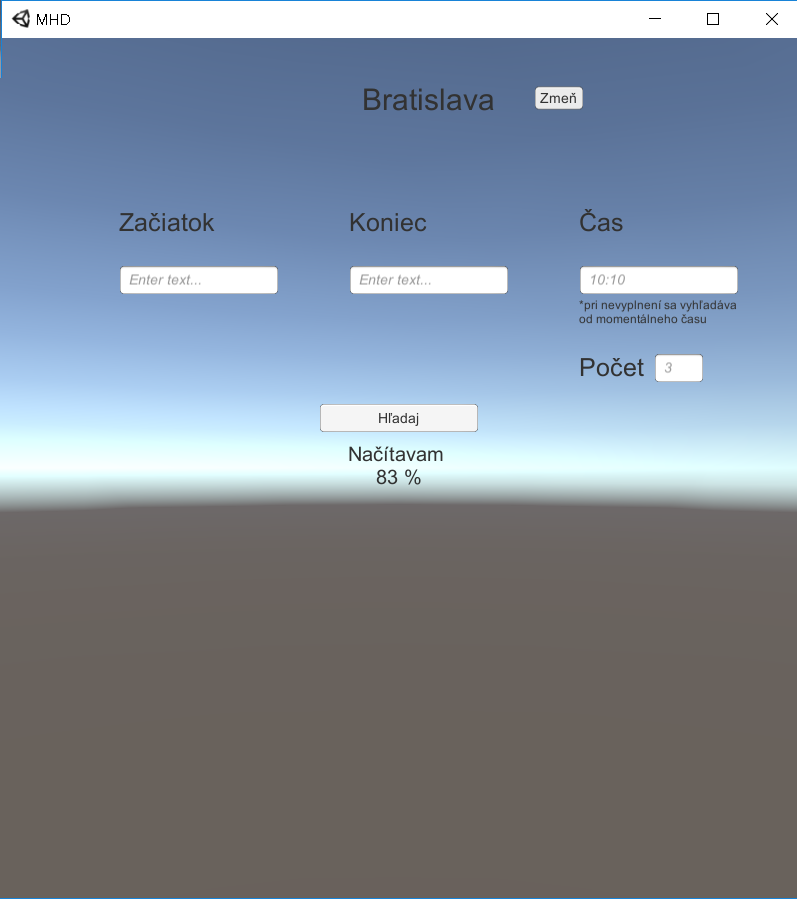
\includegraphics[width=0.6\linewidth]{./images/ukazka_programu1.png}}
  \caption{Ukážka spusteného programu}
  \label{ukazka_programu1}
\end{figure}

Na obrázku \ref{ukazka_programu1}, možno vidieť textové polia pod textami \textit{Začiatok} a \textit{Koniec}, ktoré použijú zadaný text ako začiatočný a koncový bod pre vyhľadávací algoritmus. Upozorňujeme, že názvy zastávok musia byť zadané presne tak, ako sú uložené v internej databáze, teda v textovom súbore, ktorý neskôr popíšeme.\newline

Textové pole \textit{Čas} berie za vstup, ako je v poli naznačené, čas vo formáte "hh:mm". Ak je prvá hodnota nula, netreba ju zadávať. Správne vstupy sú napríklad "5:32", "17:08"  či "9:2". Ak bude formát vstupu zlý, prípadne používateľ nechá pole prázdne, vyhľadávanie začne v momentálnom čase, aký je nastavený na používanom zariadení.\newline

Pole \textit{Počet} požaduje vyplniť číslo, ktoré určí, koľko výsledkov sa má najviac zobraziť. Opäť, pri nesprávnom vstupe či nevyplnenom poli sa použije hodnota $3$.\newline

Tlačidlo \textit{Hľadaj} spracuje vstupné údaje a spustí s nimi vyhľadávanie.\newline


\section{Vyhľadávanie}

Funkčnosť vyhľadávania ukážeme na jednom z našich testových vstupov. Nech je vstupný grafikon rovnaký ako na obrázku \ref{priklad_vstupu_softver} a uvažujme linku '1' vyrážajúcu z $A$ cez $B$ do $C$ v časoch 0:1 a 0:5 a linku '2' v čase 0:1 premávajúci iba z $A$ do $C$.\newline

\begin{figure}[H]
  \centering{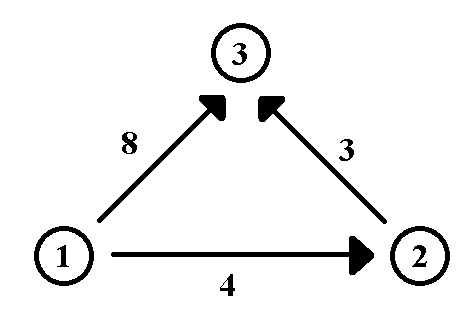
\includegraphics{./images/dijkstra_priklad.png}}
  \caption{Príklad testového vstupu}
  \label{priklad_vstupu_softver}
\end{figure}

Spustime teda vyhľadávanie z $A$ do $C$ v čase 0:0. Vidieť, že sa do požadovanej zastávky môžeme dostať v časoch 0:9 a 0:12. Možno si povšimnúť, že linka '1' i linka '2' prídu obe v čase 0:9 do koncovej zastávky.\newline

\begin{figure}[H]
  \centering{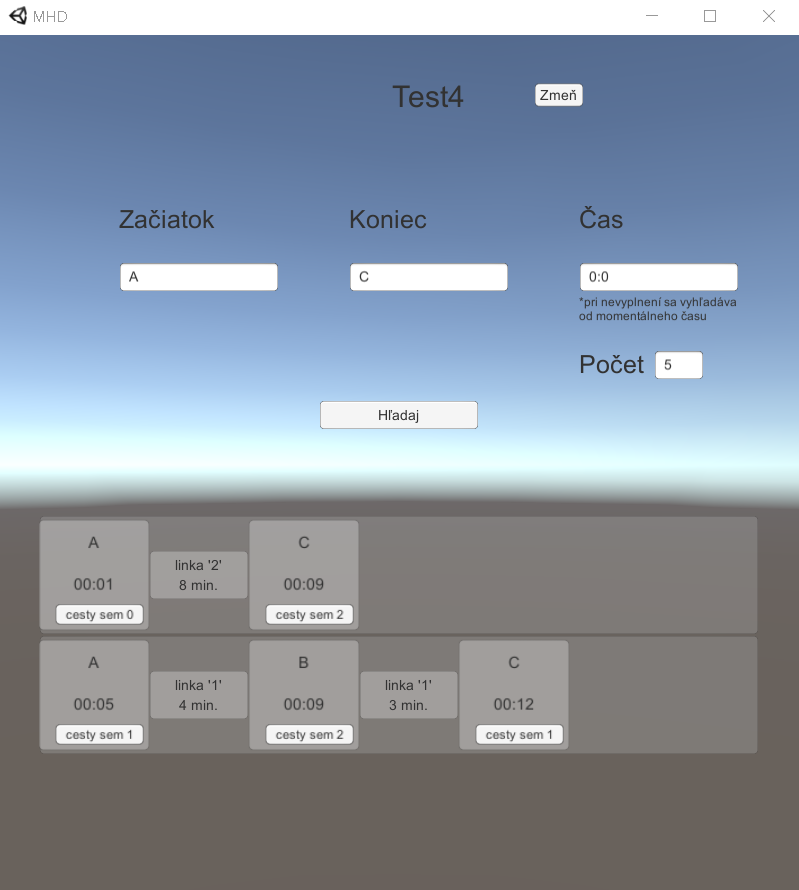
\includegraphics[width=0.6\linewidth]{./images/ukazka_programu2.png}}
  \caption{Ukážka vyhľadávania}
  \label{ukazka_programu2}
\end{figure}

Vidíme, že výsledok vyhľadávania aplikácie je správny. Navyše, pri zastávke $C$ v čase 0:9 je tlačidlo \textit{cesty sem 2}, ktoré naznačuje, že existujú, ako sme i my usúdili, dve relevantné cesty do tejto zastávky v tom istom čase. Po kliknutí na tlačidlo sa obe zobrazia spolu s tlačidlom \textit{Naspäť}, ktoré zobrazí predošlé výsledky.\newline

\begin{figure}[H]
  \centering{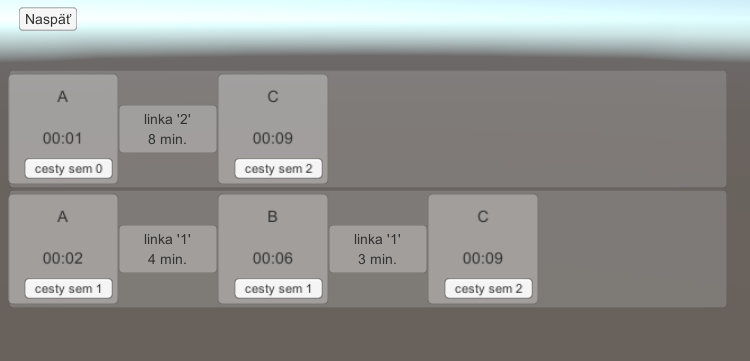
\includegraphics[width=0.6\linewidth]{./images/ukazka_programu2-alt.png}}
  \caption{Ukážka alternatívnej cesty do zastávky C}
  \label{ukazka_programu2_alt}
\end{figure}


\section{Chybové hlásenia}

Aplikácia je skonštruovaná tak, aby chyby, ktoré nastanú počas behu programu a sú pravdepodobne zapríčinené používateľom, vypísala hneď pod tlačidlo \textit{Hľadaj} spolu s radou, ktorá by mohla chybu odstrániť.\newline

\begin{figure}[H]
  \centering{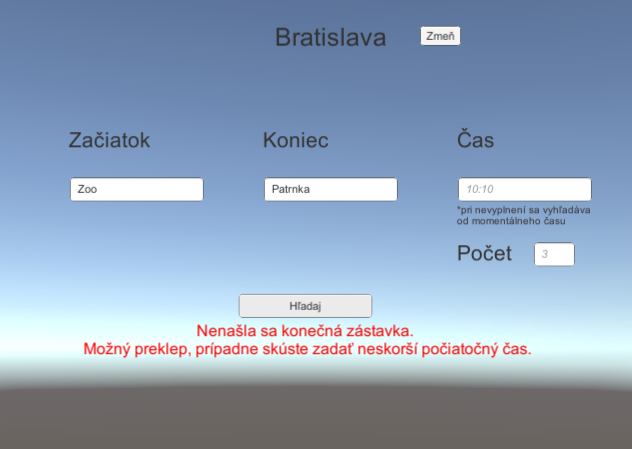
\includegraphics[width=0.6\linewidth]{./images/ukazka_programu-chyba.png}}
  \caption{Ukážka výpisu chybovej hlášky}
  \label{ukazka_chyby}
\end{figure}


\section{Dátové súbory}

Naša aplikácia je konštruovaná tak, aby si každý jej požívateľ mohol vytvoriť vlastné dáta, s ktorými má pracovať.\newline

Zložka so spustiteľným súborom aplikácie obsahuje i zložku \textit{MHD\_Data} a tá zložku \textit{Data}. V nej sa nachádzajú rôzne testové vstupy. Stačí teda vytvoriť zložku s príznačným názvom a do nej umiestniť dva textové súbory s názvami \textit{zastavky} a \textit{linky}. Súbor \textit{zastavky} má obsahovať názvy všetkých zastávok. Súbor \textit{linky} je trochu zložitejší. Ten obsahuje linky, pričom každú popisuje 5 riadkov súboru. V prvom je názov linky. Zvyšné štyri sú rozdelené - prvé dva značia cestu linky tam, druhé dva cestu linky naspäť. Tieto dva a dva riadky majú rovnaký formát, preto z nich popíšeme len jednu dvojicu. V prvom riadku z dvoch sa nachádza vždy čas od počiatočnej zastávky sem a názov zastávky v chronologickom poradí. Táto dvojica času a názvu je od ďalšej oddelená znakom $|$ . Druhý riadok obsahuje časy, v ktorých linka vyráža z počiatočnej zastávky. Formát tohto súboru sa môže javiť mierne chaotický, preto uvádzame i obrázok \ref{Format_datoveho_suboru1}, ktorý ho názorne popisuje.\newline

\begin{figure}[H]
  \centering{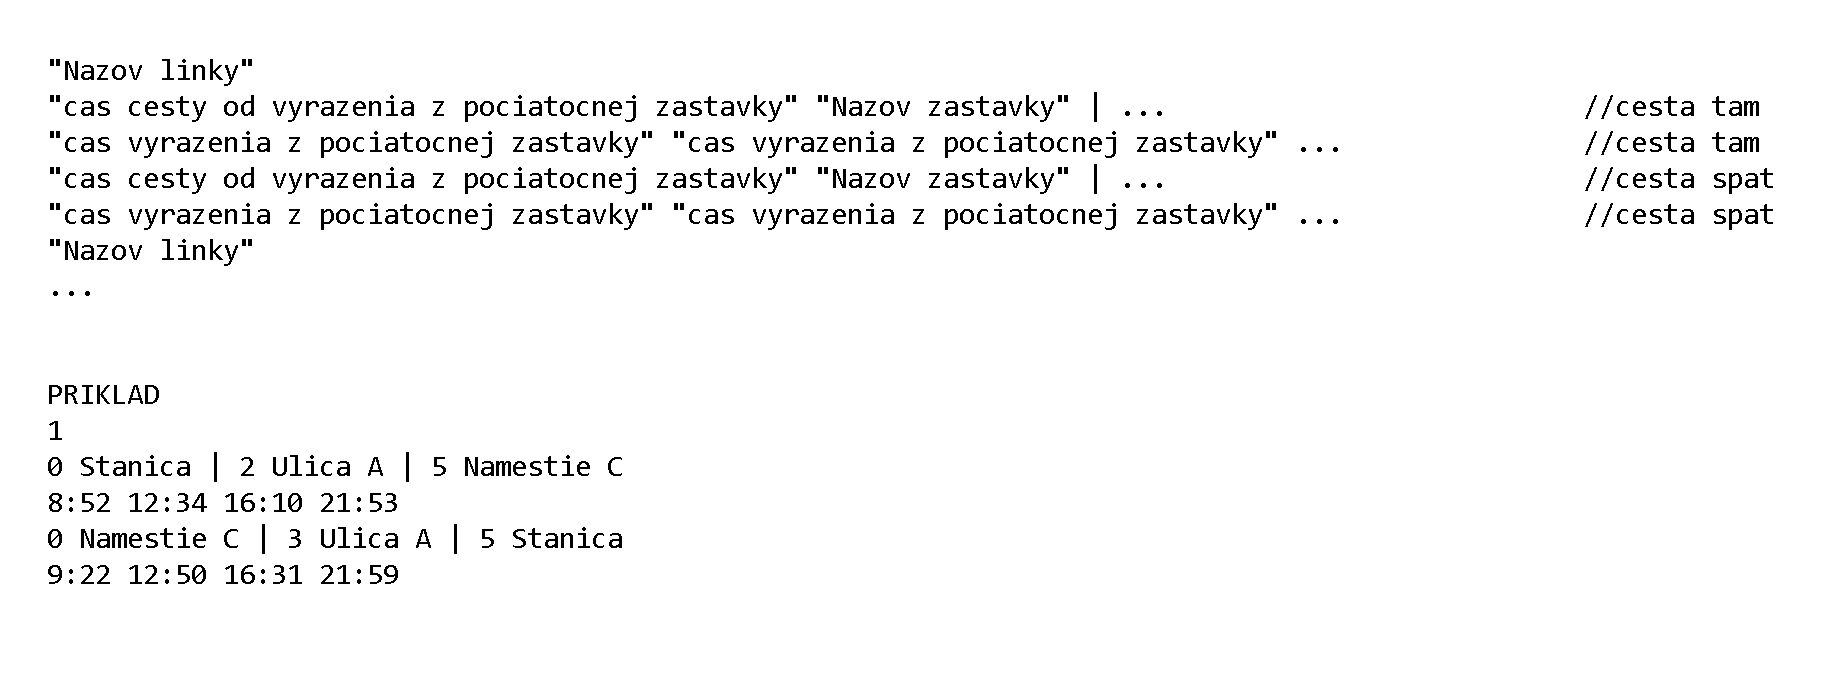
\includegraphics[width=\linewidth]{./images/Format_datoveho_suboru.png}}
  \caption{Formát dátového súboru pre linky}
  \label{Format_datoveho_suboru1}
\end{figure}

Po vytvorení zložky s dátami už stačí len v programe kliknúť na tlačidlo \textit{Zmeň}, čo zobrazí textové pole, do ktorého používateľ zadá názov vytvorenej zložky a klikne na to isté tlačidlo (teraz už s nápisom \textit{OK}). Program sa následne postará o načítanie dátových súborov, čo zapríčiní i zmenu textu hneď vedľa spomínaného tlačidla na názov poskytnutej zložky.\newline

\begin{figure}[H]
  \centering{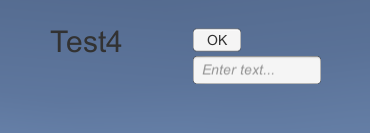
\includegraphics{./images/ukazka_programu3.png}}
  \caption{Zmena dát, s ktorými má program pracovať}
  \label{ukazka_programu3}
\end{figure}
